\documentclass[tikz,border=8pt]{standalone}
% Shared look for every TikZ diagram. Load with \input{../../tools/tikz-style.tex}
\usepackage[sfdefault]{roboto}
\usetikzlibrary{arrows.meta, positioning, shapes.geometric, calc, fit, backgrounds}
\definecolor{cblue}{HTML}{4C78A8}
\definecolor{corange}{HTML}{F58518}
\definecolor{cgreen}{HTML}{54A24B}
\definecolor{cred}{HTML}{E45756}
\definecolor{cpurple}{HTML}{B279A2}
\definecolor{cgrey}{HTML}{6B6B6B}
\tikzset{
  every picture/.style={font=\sffamily, line width=1.2pt},
  box/.style={draw=#1, fill=#1!12, rounded corners=4pt, align=center, inner sep=7pt, minimum height=1.1cm},
  box/.default=cgrey,
  arrow/.style={-{Stealth[length=3mm]}, draw=cgrey, line width=1.4pt},
  title/.style={font=\sffamily\bfseries\Large},
  note/.style={font=\sffamily\small, text=cgrey, align=center},
}
\AtBeginDocument{\hyphenpenalty=10000 \exhyphenpenalty=10000}

% The three numbers of the polar-coordinate pose controller at the start: rho (distance to the dock point),
% alpha (heading to line of sight), beta (line of sight to the dock heading), with the numbers of the Note.
\begin{document}
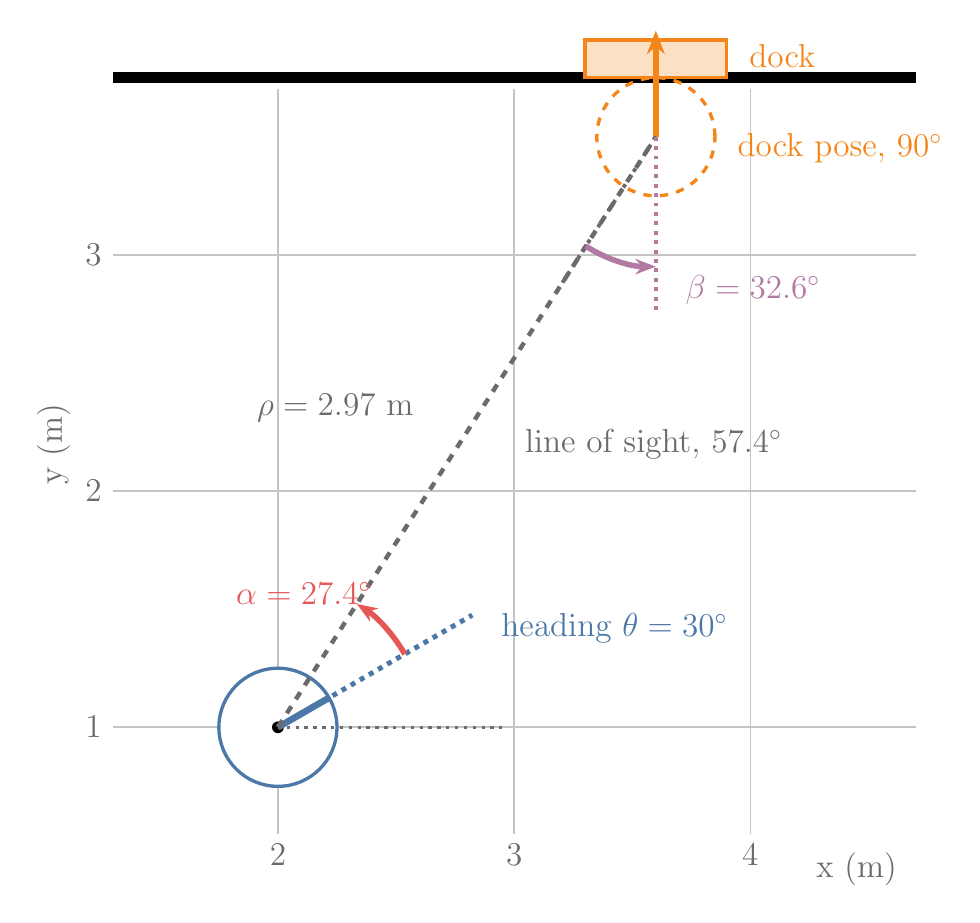
\begin{tikzpicture}[scale=3.0, every node/.append style={font=\large}]
  % wall and dock
  \draw[line width=4pt] (1.3,3.75) -- (4.7,3.75);
  \draw[corange, fill=corange!25] (3.3,3.75) rectangle (3.9,3.91);
  \node[corange, anchor=west] at (3.95,3.84) {dock};
  % floor grid ticks
  \foreach \x in {2,3,4} \draw[cgrey!40, line width=0.6pt] (\x,0.55) -- (\x,3.7);
  \foreach \y in {1,2,3} \draw[cgrey!40, line width=0.6pt] (1.3,\y) -- (4.7,\y);
  \foreach \x in {2,3,4} \node[cgrey, below] at (\x,0.55) {\x};
  \foreach \y in {1,2,3} \node[cgrey, left] at (1.3,\y) {\y};
  \node[cgrey] at (4.45,0.4) {x (m)};
  \node[cgrey, rotate=90] at (1.05,2.2) {y (m)};
  % goal pose
  \draw[corange, dashed] (3.6,3.5) circle (0.25);
  \draw[-{Stealth[length=3mm]}, corange, line width=2pt] (3.6,3.5) -- (3.6,3.95);
  \node[corange, anchor=west] at (3.9,3.45) {dock pose, $90^\circ$};
  % robot
  \draw[cblue, fill=white] (2,1) circle (0.25);
  \fill[black] (2,1) circle (0.025);
  % heading (dotted, continued) and x direction
  \draw[cblue, dotted, line width=1.8pt] (2,1) -- ++(30:0.95);
  \draw[cblue, line width=2.4pt] (2,1) -- ++(30:0.25);
  \draw[cgrey, dotted, line width=1.2pt] (2,1) -- ++(0:0.95);
  \node[cblue, anchor=west] at (2.9,1.42) {heading $\theta = 30^\circ$};
  % line of sight and rho
  \draw[cgrey, dashed, line width=1.6pt] (2,1) -- (3.6,3.5);
  \node[cgrey, anchor=east] at (2.62,2.35) {$\rho = 2.97$ m};
  % alpha arc at the robot
  \draw[-{Stealth[length=2.6mm]}, cred, line width=2pt] ($(2,1)+(30:0.62)$) arc (30:57.38:0.62);
  \node[cred, anchor=east] at ($(2,1)+(52:0.72)$) {$\alpha = 27.4^\circ$};
  % beta arc at the goal, on the floor side: line of sight and dock heading both continued back through the goal
  \draw[cgrey, dotted, line width=1.4pt] (3.6,3.5) -- ++(237.38:0.75);
  \draw[cpurple, dotted, line width=1.4pt] (3.6,3.5) -- ++(270:0.75);
  \draw[-{Stealth[length=2.6mm]}, cpurple, line width=2pt] ($(3.6,3.5)+(237.38:0.55)$) arc (237.38:270:0.55);
  \node[cpurple, anchor=west] at (3.68,2.85) {$\beta = 32.6^\circ$};
  % line of sight direction note
  \node[cgrey, anchor=west] at (3.0,2.2) {line of sight, $57.4^\circ$};
\end{tikzpicture}
\end{document}
